\documentclass[../main.tex]{subfiles}
\begin{document}
\chapter{Estado del Arte}
\section{Ortoferritas de Tierras Raras}
Los óxidos de tipo perovskita (\ce{ABO3} con A una tierra rara o metal alcalinotérreo y B un metal de transición) son estructuras estudiadas muy comúnmente en el campo de la ciencia de materiales debido a sus propiedades electromagnéticas, ópticas y catalíticas, además de su estabilidad \cite{Wang2019}.

El objeto de estudio de este trabajo son las ortoferritas \ce{RFeO3}, con R una tierra rara, específicamente \ce{R = Nd, Sm}, debido a que presentan un orden magnético intrínseco proveniente de su estructura cristalina, la cual se observa en la figura \ref{fig:estructuras}. 

Esta estructura, con grupo espacial Pbnm, es decir, una celda primitiva ortorrómbica, un plano de deslizamiento tipo b, el cual es perpendicular al eje $\hat{a}$, un plano de deslizamiento tipo n, el cual es perpendicular a $\hat{b}$ y un plano de reflexión perpendicular al eje $\hat{c}$.

La geometría de esta misma estructura favorece también la aparición de momentos dipolares en las celdas cristalinas, lo hace posible la presencia de ferroelectricidad, haciendo de estas ferritas posibles materiales multiferroicos. \cite{Sharma2024}.
\begin{figure}[H]
    \centering
    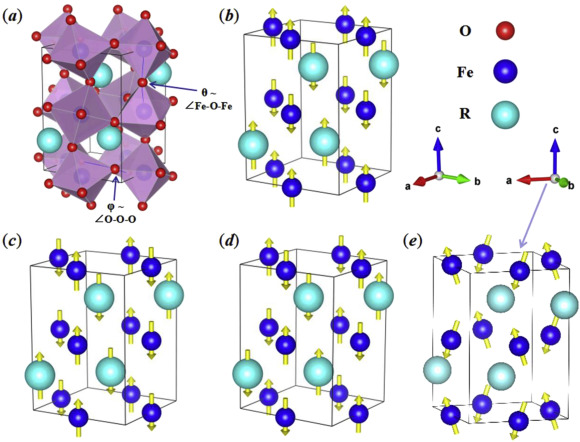
\includegraphics[width=0.5\textwidth]{fig/estructura.jpg}
    \caption{Estructura y posibles alineaciones de las subredes magnéticas de los compuestos \ce{RFeO3}. Tomado de \cite{Wang2019}}
    \label{fig:estructuras}
\end{figure}

Como se observa en la figura \ref{fig:estructuras} (a), la estructura puede pensarse como una red de octahedros de \ce{FeO6}, superpuesta a una red de átomos de \ce{R}. El ángulo formado por los enlaces \ce{Fe}-\ce{O}-\ce{Fe} es dependiente del radio iónico de \ce{R}, siendo la temperatura de Néel, que se discutirá a detalle en la sección \ref{sec:magtemp}, dependiente de ambos parámetros, como se muestra en la figura \ref{fig:neelradio}.

\begin{figure}[H]
    \centering
    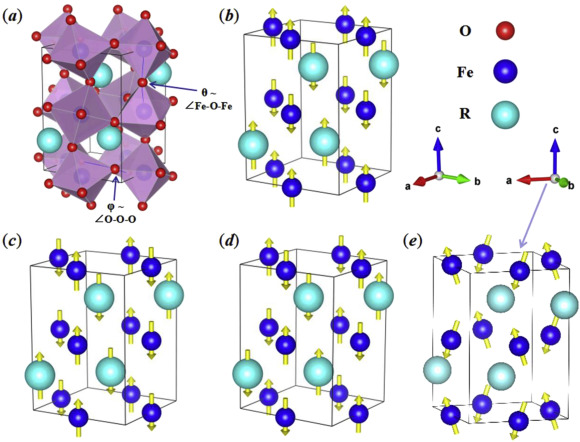
\includegraphics[width=0.5\textwidth]{fig/estructura.jpg}
    \caption{CAMBIAR FIGURA, PAPER WANG FIG 2. Relación entre el radio iónico de \ce{R}, el ángulo formado por los enlaces \ce{Fe}-\ce{O}-\ce{Fe} y la temperatura de Néel. Tomado de \cite{Wang2019}}
    \label{fig:neelradio}
\end{figure}

\section{Electromagnetismo en Sólidos}
La respuesta de un sólido al aplicar un campo externo, sea éste magnético o eléctrico, depende de las propiedades intrínsecas de la estructura cristalina de éste. A pesar de esto, las interacciones a nivel cuántico se manifiestan macroscópicamente como propiedades extensivas, las cuales pueden estudiarse mediante la electrodinámica clásica.

Las ecuaciones de Maxwell pueden modificarse para incluir las contribuciones dependientes de las propiedades del material, considerando que las cargas y corrientes dentro de un éste pueden moverse libremente, o estar ligadas.

Así, se puede escribir:
\begin{equation}
    \begin{split}
        \vec{E}=\varepsilon_0\vec{D}-\vec{P}\\
        \vec{B}=\mu_0(\vec{H}-\vec{M})
    \end{split}  
    \label{eq:maxwellmacro}
\end{equation}
Donde la fuente de los campos $\vec{D}$ y $\vec{H}$ son las cargas (o corrientes) libres, determinadas por la configuración del sistema, mientras que para los campos $\vec{P}$ y $\vec{M}$ son las cargas (o corrientes) ligadas, determinadas por las propiedades del material \cite{griffiths2023introduction}.
\subsection{Magnetización y Polarización en Sólidos}
Ambas propiedades representan la respuesta de la estructura a los campos externos. Macroscópicamente, pueden escribirse de la siguiente manera:
\begin{equation}
    \begin{split}
        P_{i}=\varepsilon_0\chi_{ij}^{(e)}E_j\\
        M_{i}=\chi_{ij}^{(m)}B_j
    \end{split}
    \label{eq:tensorMP}
\end{equation}
En esta expresión, $\chi_{ij}$, la susceptibilidad, representa los componentes de un tensor de $3\times3$ \cite{Damjanovic2006}.

Sin embargo, para un material isótropo, esta relación se simplifica a una multiplicación por un escalar, el cual aún puede depender de factores como la temperatura o el tiempo.
\begin{equation}
    \begin{split}
        \vec{P}=\varepsilon_0\chi^{(e)}\vec{E}\\
        \vec{M}=\chi^{(m)}\vec{B}
    \end{split}
    \label{eq:escalarMP}
\end{equation}
Por otro lado, también es posible entenderlas como la suma de una propiedad microscópica, es decir, para un volumen de material $V$ pueden escribirse como:
\begin{equation}
    \begin{split}
        \vec{P}=\sum_i \dfrac{\vec{d_i}}{V}\\
        \vec{M}=\sum_i \dfrac{\vec{m_i}}{V}
    \end{split}
    \label{eq:relacionmicromacro}
\end{equation}
Donde $\vec{m_i}$ es el momento magnético de cada electrón en el material, y $\vec{d_i}$ es el momento dipolar de cada celda unitaria \cite{Visintin2006}.
\subsection{Magnetización en sólidos}
Esta propiedad depende de las contribuciones de los momentos magnéticos $\vec{m_i}$ de cada electrón dentro del volumen estudiado $V$, es decir:
\begin{equation}
    \vec{M}=\sum_i\dfrac{\vec{m_i}}{V}
    \label{eq:micromag}
\end{equation}
Macroscópicamente, se puede observar que el campo de magnetización depende del campo aplicado $\vec{B}$ y de la susceptibilidad, la cual es un tensor con componentes $\chi_{ij}$, es decir:
\begin{equation}
    M_j=\chi_{ij}B_i
    \label{eq:tensormag}
\end{equation}
Para materiales en los que $\chi_{ij}=\chi\delta_{ij}$, es decir, el tensor de susceptibilidad es diagonal, se puede escribir:
\begin{equation}
    \vec{M}=\chi\vec{B}
    \label{eq:macromag}
\end{equation}
Al medir la magnetización de muestras policristalinas, o muestras en polvo, se miden simultáneamente todas las direcciones, debido a las diversas orientaciones de cada cristal. Esto arroja un promedio escalar de manera similar a la ecuación \ref{eq:macromag}, perdiendo en el proceso información sobre la dependencia direccional de la magnetización \cite{Mugiraneza2022}.
\subsubsection{Clasificación de Materiales Magnéticos}
Pueden dividirse en dos grupos de acuerdo a su comportamiento magnético, aquellos cuya respuesta magnética depende de su interacción con el campo externo y aquellos que presentan un orden magnético intrínseco. El primer grupo se compone de los siguientes materiales:
\begin{itemize}
    \item \textbf{Diamagnéticos:} Para un electrón sujeto a una órbita al cual se le aplica un campo magnético externo, la torca que éste ejerce sobre el momento magnético del electrón provoca un efecto conocido como la Precesión de Larmor, el cual consiste en una rotación periódica en el momento magnético. Ésto puede verse como una corriente que, debido a la Ley de Lens, provocará un campo magnético que se opone al campo que la generó, es decir, $\chi<0$ \cite{coey2010magnetism}.
    \item \textbf{Paramagnetismo:} Cuando un material que posee electrones desapareados en su capa de valencia es expuesto a un campo magnético externo ($H$), favorecerá el alineamiento de los momentos magnéticos de cada electrón en el mismo eje. En particular, para los electrones desapareados, el campo favorecerá a la población paralela sobre la antiparalela, provocando una magnetización en el mismo sentido que el campo externo, es decir, $\chi>0$, siendo $\chi$ constante a campos pequeños, pero llegando a una saturación cuando todos los momentos se han alineado. Sin embargo, al retirar el campo externo, estos momentos magnéticos volverán a orientarse de forma aleatoria, regresando la magnetización a 0 \cite{coey2010magnetism}.
\end{itemize}
Por otro lado, el segundo grupo se caracteriza por poseer orden magnético intrínseco, esto debido a las interacciones de intercambio entre átomos. Cuando se tiene un enlace metálico, los electrones de la red pueden moverse libremente a en un orbital que comparten todos los átomos de la red. Esto produce una degeneración en la energía, debido a que debe haber más de dos electrones en este orbital.

Los electrones en este estado pueden decaer a estados energéticos más bajos en cualquier átomo en la red, produciendo un intercambio entre ellos.

Este comportamiento puede modelarse mediante el siguiente hamiltoniano:
\begin{equation}
    \mathcal{H}_{\text{Heisenberg}}=-2\mathcal{J}\vec{S_i}\vec{S_j}
    \label{eq:heisenberginterc}
\end{equation}
Donde $\mathcal{H}_{\text{Heisenberg}}$ se conoce como el hamiltoniano de Heisenberg, $\mathcal{J}$ es una constante que depende de la estructura del cristal y $\vec{S_i}$ y $\vec{S_j}$ son los espines totales de dos átomos consecutivos \cite{coey2010magnetism}.

Según el signo de $\mathcal{J}$ se favorece un acomodo paralelo ($\mathcal{J}>0$) o antiparalelo ($\mathcal{J}<0$) de los espines. Esto produce zonas dentro del material cuyos electrones poseen espines alineados, conocidos como dominios magnéticos. Esto es lo que da lugar a los 3 tipos de material con orden magnético intrínseco:
\begin{itemize}
    \item \textbf{Ferromagnéticos ($\mathcal{J}>0$):} Los espines se alinean de forma paralela debido al signo de $\mathcal{J}$, esto provoca que los dominios magnéticos tengan una magnetización distinta de 0. Cuando se aplica un campo magnético externo $H$, los dominios cuya magnetización es paralela a $H$ comienzan a crecer a costa de las zonas con magnetizaciones en direcciones distintas. Son similares a los materiales paramagnéticos debido a que ambos provienen de una reorientación de espines, ambos tienen una $\chi>0$, y ambos poseen un campo de saturación $M_s$, sin embargo, la interacción de intercambio provoca un campo de magnetización remanente $M_r$ incluso al retirar el campo externo, para regresar la magnetización a 0 es necesario aplicar un campo coercitivo $H_c$ \cite{coey2010magnetism}.
    \item \textbf{Antiferromagnéticos ($\mathcal{J}<0$):} De manera similar a los materiales ferromagnéticos, estos también presentan dominios magnéticos, sin embargo, los espines se alinean de forma antiparalela, puesto que $\mathcal{J}<0$, esto genera dos subredes, cuyos espines apuntan en direcciones opuestas, sin embargo, la magnetización generada por ambas subredes es de la misma magnitud, es decir, la magnetización neta es 0 \cite{coey2010magnetism}.
    \item \textbf{Ferrimagnéticos $\mathcal{J}<0$:} Finalmente, los materiales ferrimagnéticos son similares a los antiferromagnéticos, también forman dos subredes con espines alineados en direcciones opuestas, sin embargo, la magnetización de una subred es mayor que la de la otra, lo cual provoca una magnetización neta positiva, aunque menor a la de los materiales ferrimagnéticos \cite{coey2010magnetism}.
\end{itemize}
\subsubsection{Transiciones de Fase Magnéticas} \label{sec:magtemp}
Debido a que la magnetización se compone de la suma de efectos a nivel cuántico, es de esperarse que tenga dependencia en la temperatura.

La única excepción es el diamagnetismo, 
\subsection{Histéresis} \label{sec:hist}
Un fenómeno presenta histéresis si depende no sólo de las condiciones actuales del sistema, sino que también de las condiciones anteriores. Ésto ocurre para propiedades como la elasticidad, la fricción, la superconductividad, la adsorción, la desorción y, siendo éstas el objeto de estudio de este trabajo, la magnetización y la polarización.

En general, la histéresis, observada en propiedades extensivas, proviene de las contribuciones microscópicas de propiedades intensivas \cite{Visintin2006}.

Este fenómeno es evidente al aplicar un campo externo, sea este magnético o eléctrico, los dominios en el material cuya propiedad intensiva relevante sea paralela al campo aplicado serán energéticamente favorables y por lo tanto crecerán a costa de aquellos dominios orientados de forma distinta, lo que aumenta la propiedad extensiva relevante hasta alcanzar un valor máximo, conocido como campo de saturación.

Este proceso no es reversible, si se quita el campo externo el sistema no regresará por si solo a la configuración inicial, sino que tendrá una polarización, o magnetización, remanente distinta de 0. Si se busca que ésta se anule, se debe de aplicar un campo externo en sentido opuesto, conocido como campo coercitivo.
\subsection{Clasificación de Materiales}
Es posible clasificar los materiales según su respuesta a los campos externos aplicados.

Hasta ahora ambos campos han tenido relaciones análogas, sin embargo, el hecho de que sólo el campo eléctrico posea cargas, hace que existan comportamientos de la polarización que no se observan para la magnetización. Por esta razón, se discutirán por separado.

\subsubsection{Clasificación de Materiales Eléctricos}
\subsection{Multiferroicidad}
\end{document}